\chapter{Making Figures or Images Accessible} \label{ch:graphics}

\section{Accessible Figures and the Role of Alt-Text}
To ensure that figures and images are accessible to users who rely on screen readers and other assistive technologies, all non-decorative visual content must be accompanied by \textit{meaningful} alternative text (alt-text).
Alt-text provides a textual representation of visual information and enables users who cannot perceive images visually to understand their purpose and content.

Alt-text should concisely describe the essential information conveyed by the figure, focusing on what a user needs to know rather than how the image looks.
The description should be written in complete sentences or clear phrases and should avoid redundant wording such as ``an image of'' or ``a figure showing,'' as screen readers already announce the presence of an image.
For informative figures (\textit{e.g.}, diagrams, plots, flowcharts, screenshots, or visual comparisons), the alt-text should summarize the key message or insight conveyed by the figure.
When a figure contains text, labels, or numerical values that are critical for understanding, these should be included or summarized in the alt-text.
If the figure is complex and cannot be adequately described in a short alt-text, an abridged version should be provided along with a more detailed explanation in the surrounding text or caption.

\section{Providing Alt-Text for Simple Figures}

Documentation on how to generate alt-text for graphics in \LaTeX\ can be found in the \href{https://texdoc.org/serve/latex-lab-graphic/0}{latex-lab-graphic package manual}; however, we will demonstrate some basic examples in this template.
To include an image and embed with it alternative text, we may use the \verb|\includegraphics{}| command and leverage the \verb|alt={}| key.
This is demonstrated in \autoref{fig:alt-text}, which depicts the code used to generate the image itself, visually identifying where the alt-text should be placed.

\begin{figure}[ht]
  \centering
  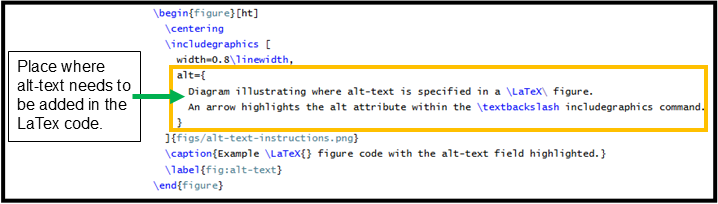
\includegraphics [
    width=0.8\linewidth,
    alt={
      Diagram illustrating where alt-text is specified in a \LaTeX\ figure.
      An arrow highlights the alt attribute within the \backslash includegraphics command.
    }
  ]{figs/alt-text-instructions.png}
  \caption{Example \LaTeX\ figure code with the alt-text field highlighted}
  \label{fig:alt-text}
\end{figure}

\newpage

As of October 2026, packages for \textit{generating} graphics should be used with caution: \texttt{tikz} is only partially compatible with tagging, and \texttt{pgfplots} is currently incompatible.
In general, simple graphics generated using \texttt{tikz} can be used if you provide alt-text as in \autoref{fig:parabola}.
\vspace{3em}

\begin{figure}[h]
  \centering
  \begin{tikzpicture}[
      alt={A parabola opening upward, centered at the origin (0,0).}
    ]

    \draw[->] (-2.5,0) -- (2.5,0) node[below] {$x$};
    \draw[->] (0,-0.5) -- (0,4.5) node[left] {$y$};

    \draw[thick, blue] (-2,4) parabola bend (0,0) (2,4);

  \end{tikzpicture}
  \caption{A figure generated using \texttt{tikz}}
  \label{fig:parabola}
\end{figure}

A considerably more complicated example can be found in \autoref{fig:complicated}---this example also shows how intricate figures can be \texttt{\backslash input} from a separate file, just like tables.
Refer to the documentation linked previously if you wish to generate things other than simple figures (\textit{e.g.}, decorations, special characters) using \texttt{tikz}, as these might require further care to tag properly or need to be marked as artifacts.

\begin{figure}[ht]
  \centering
  \begin{tikzpicture}[
      alt={A graph consisting of a path from x_0 to x_k that splits into two parallel branches (of lengths l_1 and l_2), which later rejoin at z_0 and continue to z_m.},
    roundnode/.style={circle, fill=black, inner sep=0pt, minimum size=1.75mm}]
    \node[roundnode, label=90:{$x_0$}] (x0) at (0,0) {};
    \node[roundnode, label=90:{$x_1$}] (x1) at (1,0) {};
    \node[roundnode, label=90:{$x_2$}] (x2) at (2,0) {};
    \node (p1) at (2.5,0) {\ldots};
    \node[roundnode, label=90:{$x_k$}] (xk) at (3,0) {};

    \node[roundnode, label=90:{$y_1^{(1)}$}] (y11) at (4,1) {};
    \node[roundnode, label=90:{$y_2^{(1)}$}] (y21) at (5,1) {};
    \node (p2) at (5.5,1) {\ldots};
    \node[roundnode, label=90:{$y_{l_1-1}^{(1)}$}] (yl'1) at (6,1) {};

    \node[roundnode, label=270:{$y_1^{(2)}$}] (y12) at (4,-1) {};
    \node[roundnode, label=270:{$y_2^{(2)}$}] (y22) at (5,-1) {};
    \node (p3) at (5.5,-1) {\ldots};
    \node[roundnode, label=270:{$y_{l_2-1}^{(2)}$}] (yl'2) at (6,-1) {};

    \node[roundnode, label=90:{$z_0$}] (z0) at (7,0) {};
    \node[roundnode, label=90:{$z_1$}] (z1) at (8,0) {};
    \node[roundnode, label=90:{$z_2$}] (z2) at (9,0) {};
    \node (p4) at (9.5,0) {\ldots};
    \node[roundnode, label=90:{$z_m$}] (zm) at (10,0) {};

    \node (s) at (0,-.4) {$s(L)$};
    \node (t) at (10,-.4) {$t(L)$};

    %Lines
    \draw[-] (x0) -- (x1);
    \draw[-] (x1) -- (x2);
    \draw[-] (xk) -- (y11);
    \draw[-] (xk) -- (y12);
    \draw[-] (y11) -- (y21);
    \draw[-] (y12) -- (y22);
    \draw[-] (yl'1) -- (z0);
    \draw[-] (yl'2) -- (z0);
    \draw[-] (z0) -- (z1);
    \draw[-] (z1) -- (z2);

  \end{tikzpicture}
  \caption[A $(k,l_1,l_2,m)$-Laakso graph]{A $(k,l_1,l_2,m)$-Laakso graph.}
  \label{fig:complicated}
\end{figure}

